\documentclass[11pt,a4paper]{article}
\usepackage[utf8]{inputenc}
\usepackage[T1]{fontenc}
\usepackage[english]{babel}
\usepackage[margin=2.5cm]{geometry}
\usepackage{booktabs,longtable,tabularx}
\usepackage{enumitem}
\usepackage{listings}
\usepackage{graphicx}
\usepackage[hidelinks]{hyperref}
\setlength{\emergencystretch}{3em}
\lstset{basicstyle=\ttfamily\small,breaklines=true,columns=fullflexible,frame=single}
\setlength{\parskip}{0.5em}
\setlength{\parindent}{0pt}
\title{Data Modelling and Integration\\Project P1: Heterogeneous Data Sources\\Banking Subtopic}
\author{Diogo Jorge -- 57593\\Group 13}
\date{Academic year 2026/2027\\Initial working draft -- 12 November 2026}
\begin{document}
\maketitle
\renewcommand{\abstractname}{Work Order and Declaration:}
\begin{abstract}
This part of the assignment represents the the banking subtopic of Project P1 only and
was made by Diogo Jorge. The other subtopics are the responsibility 
of others and will appear directly after
this report is finished in the same file. 
There is a GitHub repository containing the totality of work developed by both students 
and it can be found at: \url{https://github.com/Diogo-Jorge-57593/MID-P1}.

\end{abstract}

\section{Domain description and project objectives}
The first sub topic selected for project P1 is banking. The domain includes the 
data modelling part of a banking app, where customers and employees will interact
with the same data.

This contribution uses MongoDB and CSV. Its objectives are to model coherent
banking entities, provide reproducible synthetic data, define representative
queries and identify the heterogeneity that future integration must resolve.
Credit decisions are stored as sample administrative outcomes

This data modelling prototype is a very simplified version a real banking system 
made with the purpose of demonstrating the ability to model and integrate
different and heterogeneous data sources.

\section{Stakeholders and requirements}
The stakeholders below are proposed personas. No interviews or expert
validation have been conducted for this draft.
\begin{description}[style=nextline]
\item[Bank Manager] Has access to several administrative level views of the existing data, including application counts and total requested amounts by status and by responsible employee.
\item[Credit officer] Reviews requests and their status history, updates their current status based on the applicant's profile and financial information.
\item[Client] Owns one or more accounts inside the baking system, may submit or have a credit application reviewed, has access to their own account information and full transaction history.
\item[Integration developer] Needs stable identifiers, documented schemas and
consistent interpretation of dates, statuses and monetary amounts.
\item[Teacher/reviewer] Needs executable scripts, expected results and a clear
statement of each student's work.
\end{description}

\subsection{Functional requirements}
\begingroup
\renewcommand{\arraystretch}{1.2}
\begin{tabularx}{\textwidth}{@{}l >{\raggedright\arraybackslash}X c@{}}
\toprule
\textbf{ID} & \textbf{Functional requirement} & \textbf{Related use case}\\
\midrule
FR1 & The system will retrieve a list of all accounts belonging to a selected client. & UC1\\
FR2 & The system will retrieve transactions for a selected client account within a specified date range. & UC2\\
FR3 & The system shall retrieve a credit application together with the applicant's profile and recorded financial information. & UC3\\
FR4 & The system shall allow a credit officer to update the application status and record the change timestamp in the status history. & UC4\\
FR5 & The system shall calculate application counts and total requested amounts by status for a specified submission period. & UC5\\
FR6 & The system shall calculate application counts and total requested amounts by responsible employee and status for a specified submission period. & UC6\\
\bottomrule
\end{tabularx}
\endgroup

\subsection{Non-functional requirements}
\begingroup
\renewcommand{\arraystretch}{1.2}
\begin{tabularx}{\textwidth}{@{}l >{\raggedright\arraybackslash}X >{\raggedright\arraybackslash}p{4.3cm}@{}}
\toprule
\textbf{ID} & \textbf{Non-functional requirement} & \textbf{Verification}\\
\midrule
NFR1 & Entity identifiers shall be unique; account, application and transaction references shall resolve to existing entities. & Duplicate IDs rejected; reference checks report zero dangling references.\\
NFR2 & Monetary values shall retain exact decimal precision throughout storage, integration and aggregation. & Calculated totals match predefined expected decimal values.\\
NFR3 & MongoDB and CSV representations shall have documented mappings for identifiers, dates, amounts and currencies. & Valid CSV examples convert to agreed representation without information loss.\\
NFR4 & Supplied fixture data and documented commands shall reproduce expected query results. & Fresh setup produces documented outputs.\\
NFR5 & Project datasets shall contain synthetic personal information only. & Review confirms records contain no real customer information.\\
\bottomrule
\end{tabularx}
\endgroup

\subsection{Use case model}
\begingroup
\renewcommand{\arraystretch}{1.2}
\begin{tabularx}{\textwidth}{@{}l >{\raggedright\arraybackslash}p{2cm} >{\raggedright\arraybackslash}p{3.4cm} >{\raggedright\arraybackslash}X@{}}
\toprule
\textbf{ID} & \textbf{Actor} & \textbf{Use case} & \textbf{Expected result}\\
\midrule
UC1 & Client & View client account & Lists account associated with the authenticaded client\\
UC2 & Client & Consult account transactions & List movements for own account and selected period.\\
UC3 & Credit officer & Review credit application & Retrieve all pertinent information about a client and it´s credit application\\
UC4 & Credit officer & Update application status & Update the status of an application\\
UC5 & Bank Manager & Summarise appilcation status & Show application counts and total requested amounts by status for selected period, aggregate amounts in \#/money\\
UC6 & Bank Manager & Summarise employee perfomance & List employees by approved/denied/pending credits \#/value\\
\bottomrule
\end{tabularx}
\endgroup

UC2 requires CSV movements and valid MongoDB account references. The remaining
use cases concern MongoDB data. Authentication and an application user interface
remain outside the project scope.

\section{Glossary and domain constraints}

\subsection{Glossary}

\begingroup
\renewcommand{\arraystretch}{1.2}
\begin{tabularx}{\textwidth}{@{}p{3.5cm} >{\raggedright\arraybackslash}X@{}}
\toprule
Term & Description\\
\midrule
Client & Bank customer who owns accounts and may submit credit applications.\\
Account & Banking account belonging to one client, with a type, currency, opening date and status.\\
Employee & Bank employee who may be assigned to handle credit applications.\\
Credit application & Client request for credit, specifying the requested amount, repayment term and purpose. Approval does not imply disbursement.\\
Requested amount & Principal requested in a credit application, expressed in EUR; it is not an outstanding balance.\\
Application status & Current application state: \texttt{pending}, \texttt{approved} or \texttt{declined}.\\
Transaction & Dated incoming or outgoing movement recorded against a bank account in the CSV source.\\
Direction & Movement classification: \texttt{IN} for incoming funds and \texttt{OUT} for outgoing funds.\\
Transfer & Movement between two accounts, represented by two transaction records sharing a transfer identifier.\\
Investor & Investment organisation associated with funding rounds in the venture-capital source.\\
Startup & Company receiving investment and associated with monthly performance reports.\\
Funding round & Investment event linking one startup and one investor, with an amount, date and round type.\\
MRR & Monthly recurring revenue: recurring revenue attributed to a month.\\
CAC & Customer acquisition cost: cost associated with acquiring a customer.\\
Churn rate & Percentage of customers lost over the reporting period.\\
\bottomrule
\end{tabularx}
\endgroup

\subsection{Domain constraints}

\begingroup
\renewcommand{\arraystretch}{1.2}
\begin{tabularx}{\textwidth}{@{}p{3.5cm} >{\raggedright\arraybackslash}X@{}}
\toprule
Constraint & Description\\
\midrule
Account ownership & Each account belongs to exactly one existing client. Each client owns one or more accounts; joint ownership is outside the current model.\\
Application ownership & Each credit application belongs to exactly one existing client. A client may submit zero or more applications.\\
Employee assignment & An employee may handle zero or more applications. An application has zero or one assigned employee; approved and declined applications require an employee, while pending applications may be unassigned.\\
Application values & Requested amounts must be positive and repayment terms must be positive whole numbers of months. Annual income must be non-negative.\\
Allowed states & Application status is \texttt{pending}, \texttt{approved} or \texttt{declined}. Account status is \texttt{active}, \texttt{blocked} or \texttt{closed}; account type is \texttt{current} or \texttt{savings}.\\
Transaction references & Every transaction identifies exactly one existing MongoDB account. Transaction identifiers are unique within the CSV source.\\
Transaction values & Transaction amounts are positive; direction determines whether funds enter or leave the account. Banking amounts use EUR.\\
Transfer pairs & Each populated transfer identifier groups exactly two transactions on different accounts: one \texttt{OUT} and one \texttt{IN}, with matching amounts and currency. Ordinary movements have no transfer identifier.\\
Funding relationships & Each funding round references one existing startup and one existing investor through PostgreSQL foreign keys. A startup or investor may participate in multiple rounds.\\
Performance references & Each JSON startup reference must match a PostgreSQL startup identifier. This relationship requires separate validation because JSON does not enforce foreign keys.\\
Currency compatibility & JSON financial indicators use USD, whereas banking data uses EUR. SQL investment currency must be clarified before monetary comparisons or conversion.\\
Cross-domain identity & Banking clients and startups have no agreed shared identifier. Cross-subtopic queries require an explicit identity mapping.\\
Temporal interpretation & Banking submission timestamps represent UTC instants. CSV movements and funding rounds use dates; JSON indicators refer to months. Queries must account for these different time granularities.\\
\bottomrule
\end{tabularx}
\endgroup

\section{Source selection and responsibility}
The project combines two subtopics: banking and credit applications, developed
by Diogo Jorge, and venture-capital investment, developed by Oleksii Nikitenko.
Each subtopic provides two sources, giving four project sources with different
structures and access methods.

\begingroup
\renewcommand{\arraystretch}{1.2}
\begin{tabularx}{\textwidth}{@{}p{2.2cm} p{2.7cm} >{\raggedright\arraybackslash}X@{}}
\toprule
Source & Responsibility & Contents and purpose\\\midrule
MongoDB & Diogo Jorge & Client profiles, accounts, employees and credit
applications; operational banking records linked through identifiers.\\
CSV & Diogo Jorge & Account transactions, including incoming and outgoing
movements and paired internal transfers; an independent banking export.\\
PostgreSQL & Oleksii Nikitenko & Investors, startups and funding rounds;
relational investment records supporting joins and aggregate queries.\\
JSON files & Oleksii Nikitenko & Monthly startup performance indicators;
nested financial reports associated with startups in PostgreSQL.\\
\bottomrule
\end{tabularx}
\endgroup

\subsection{Banking source: MongoDB}
The database \texttt{dmi\_p1\_bank} contains four collections:
\texttt{clients}, \texttt{accounts}, \texttt{employees} and
\texttt{applications}. Documents represent individual business records;
\texttt{clientId} connects accounts and applications to clients, while the
optional \texttt{employeeId} identifies the employee handling an application.
These are identifier references rather than embedded copies of related records.
The current application document stores its current status; a status-history
structure is not implemented in this version.

MongoDB provides document storage, collection validation and indexes for these
records. Validation constrains the document structure~\cite{validation}, and
Decimal128 represents monetary values without binary floating-point
conversion~\cite{decimal}. The generated dataset contains 500 clients,
1,000 accounts, 25 employees and 750 applications: 2,275 documents in total.
The schema, loader and verification scripts are available under
\path{Diogo/database/}; loading and verification have been completed locally.

\subsection{Banking source: CSV transactions}
The transaction source remains a separate file with eight columns:
\texttt{transactionId}, \texttt{accountId}, \texttt{transferId},
\texttt{bookingDate}, \texttt{direction}, \texttt{amount},
\texttt{currency} and \texttt{description}. CSV represents a flat export that
can be exchanged and processed independently of the operational database.
Its physical convention uses UTF-8, a semicolon delimiter, dates in
\texttt{DD/MM/YYYY} format and a decimal comma for amounts.

The generated file contains 8,000 transactions: 6,000 ordinary movements and
2,000 movements forming 1,000 transfer pairs. Each \texttt{accountId}
references an account in MongoDB. A populated \texttt{transferId} groups one
outgoing and one incoming movement of the same transfer; it is empty for
ordinary movements. All generated banking amounts use EUR. Generation and
validation are implemented under \path{Diogo/dataGeneration/}; the CSV has
been generated and validated, but the cross-source query runner remains
to be implemented.

\section{Models}

\subsection{Conceptual models}

The banking conceptual model shows clients, accounts, employees and credit
applications in MongoDB, together with transactions in the CSV source.
The sources are shown together to make the account--transaction relationship
explicit.

\begin{figure}[htbp]
\centering
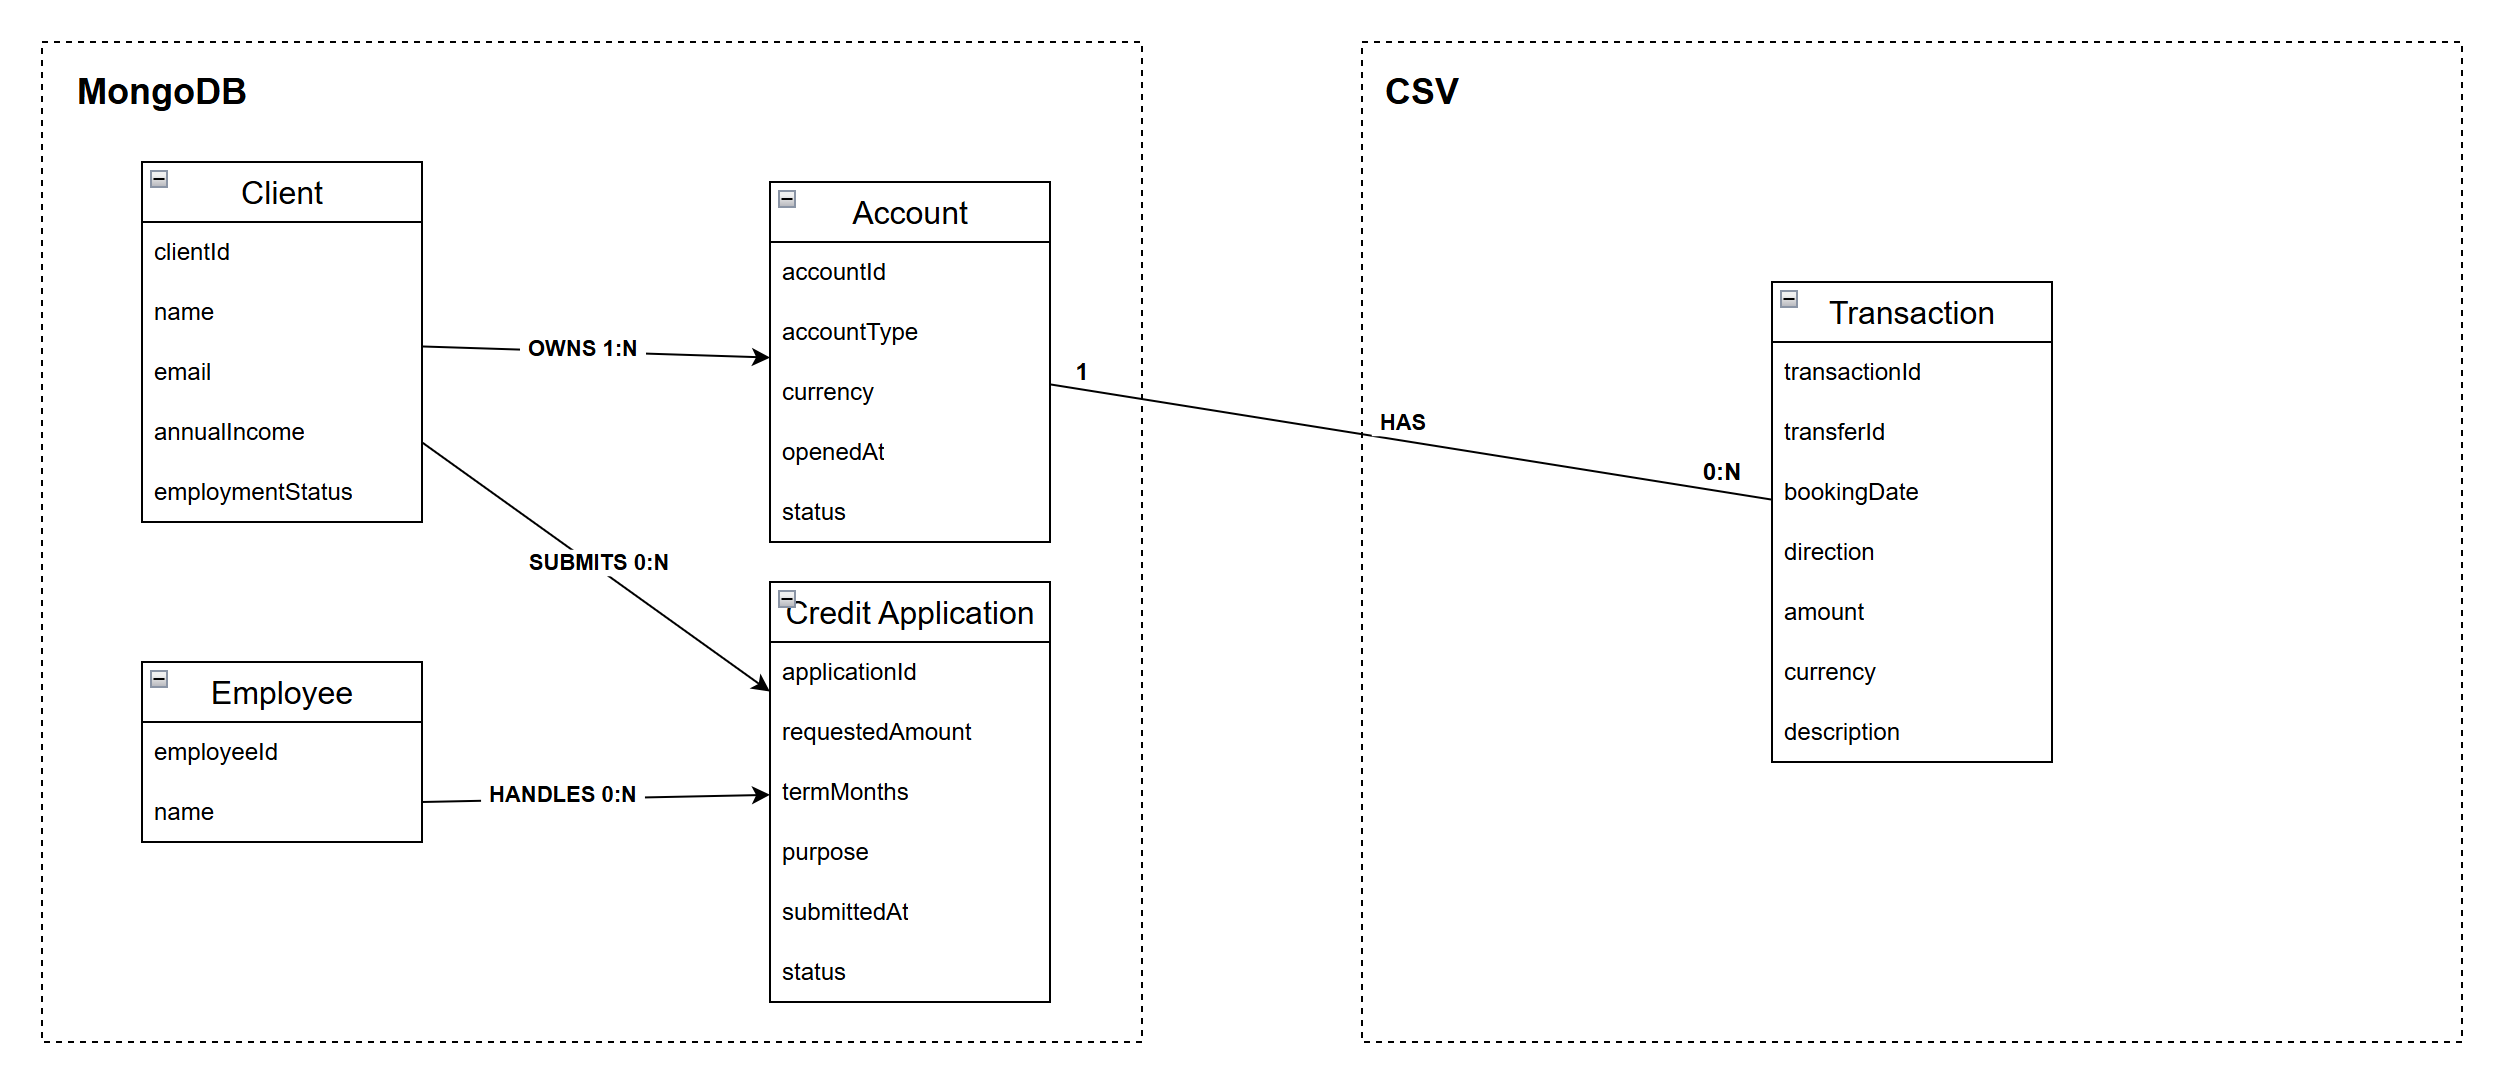
\includegraphics[width=\textwidth,height=0.70\textheight,keepaspectratio]{images/conceptual-banking.png}
\caption{Banking conceptual model: MongoDB and CSV entities and relationships.}
\label{fig:conceptual-banking}
\end{figure}
\clearpage

\subsection{Logical models}

The MongoDB logical model defines four collections and their identifier
references. Example documents illustrate the structure; the accompanying
field table specifies logical types, required fields and constraints.

\begin{figure}[htbp]
\centering
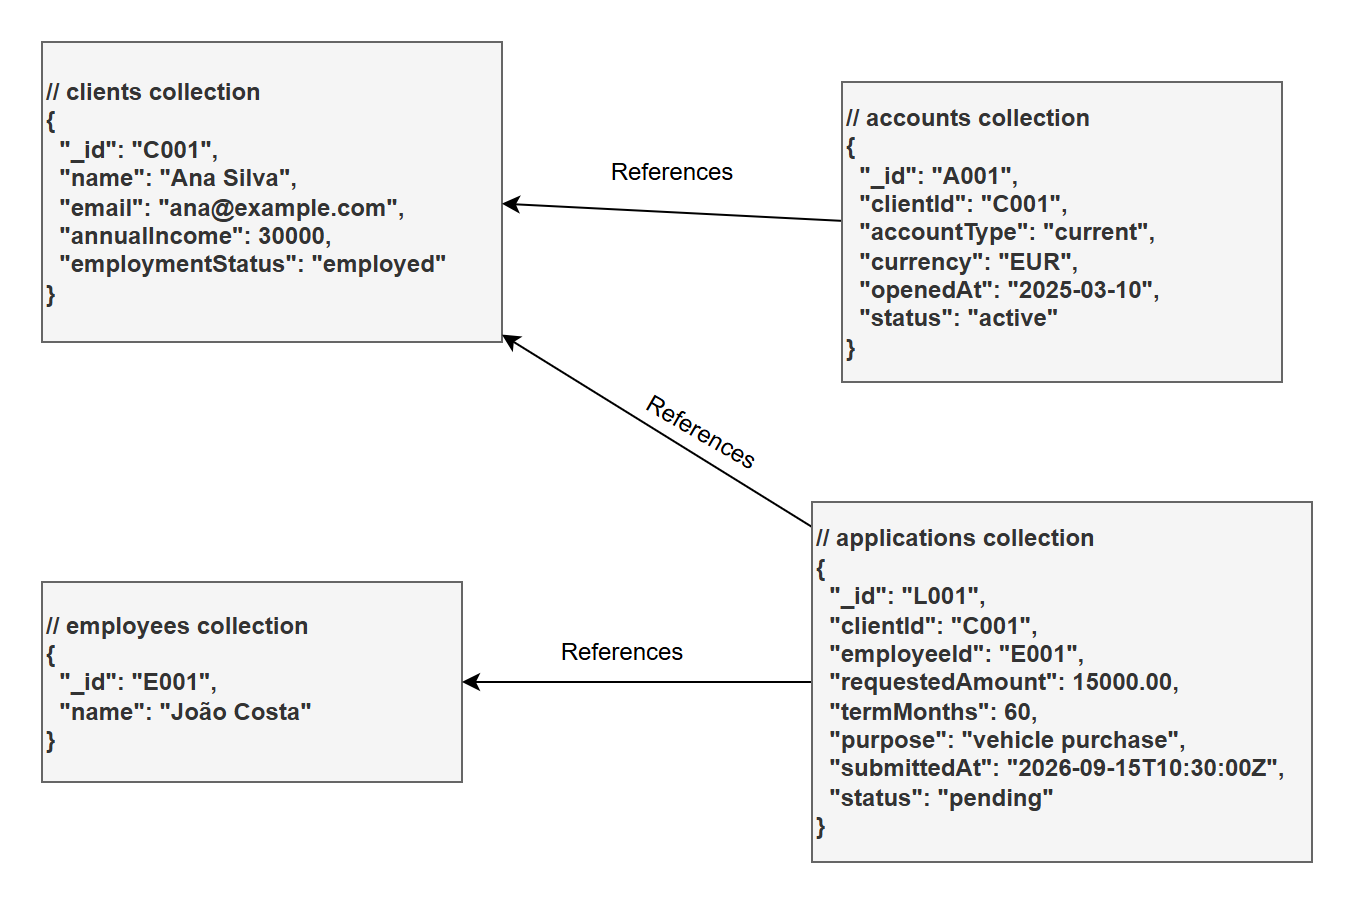
\includegraphics[width=\textwidth,height=0.68\textheight,keepaspectratio]{images/logical-mongodb.png}
\caption{MongoDB logical model: example documents and references.}
\label{fig:logical-mongodb}
\end{figure}
\clearpage

\begin{figure}[htbp]
\centering
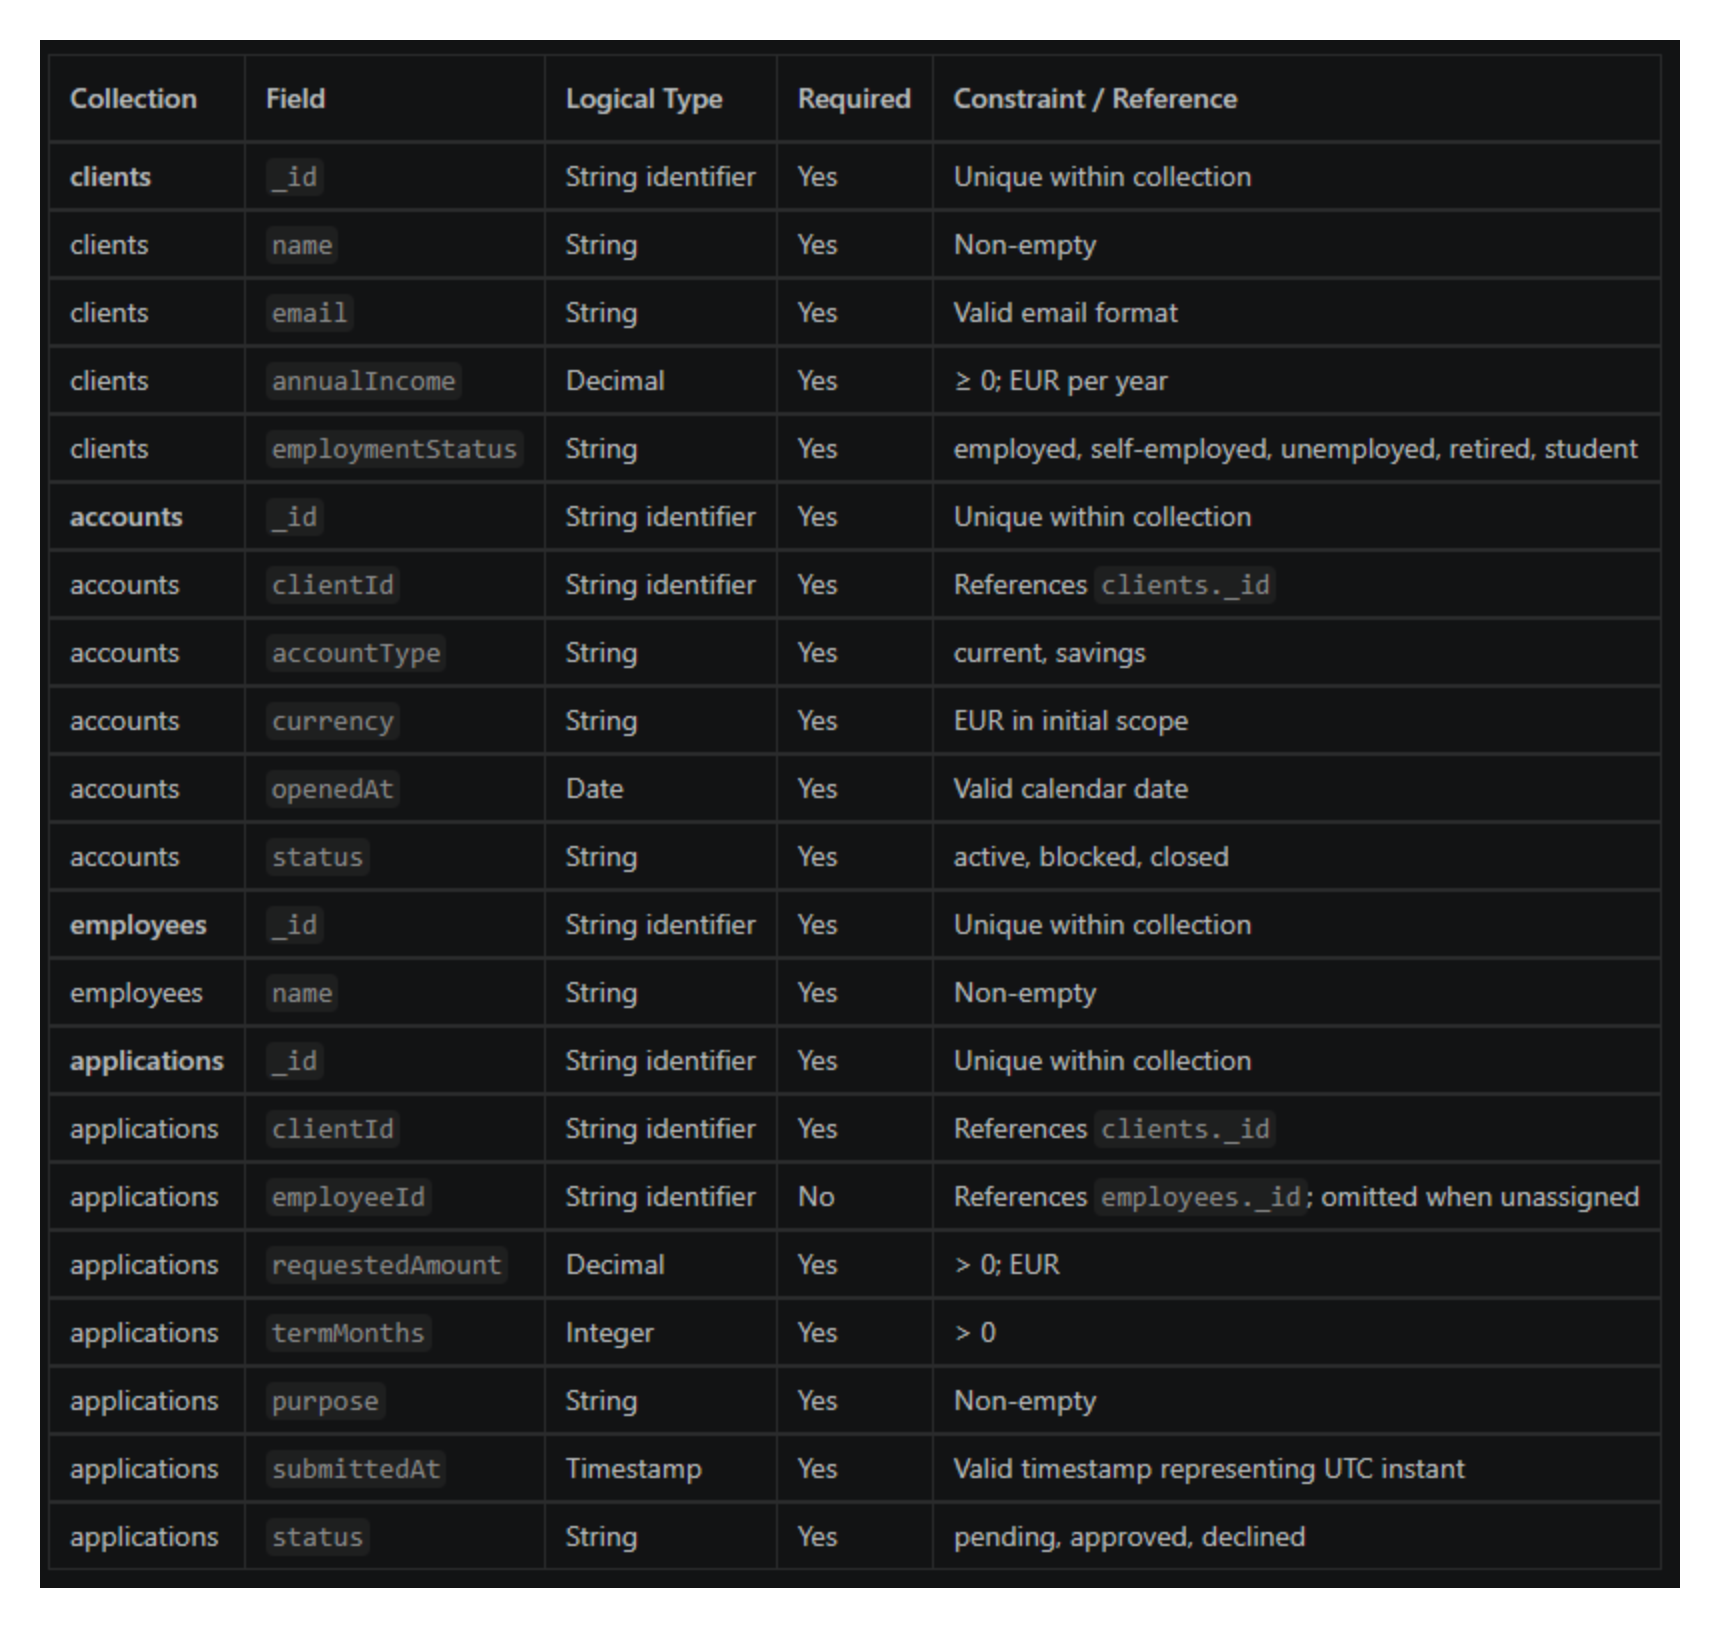
\includegraphics[width=\textwidth,height=0.85\textheight,keepaspectratio]{images/logical-mongodb-fields.png}
\caption{MongoDB logical model: field definitions and constraints.}
\label{fig:logical-mongodb-fields}
\end{figure}
\clearpage

The CSV logical model represents one transaction per record.
The field \texttt{accountId} references \texttt{accounts.\_id} in MongoDB,
while an optional \texttt{transferId} associates the two movements of a transfer.

\begin{figure}[htbp]
\centering
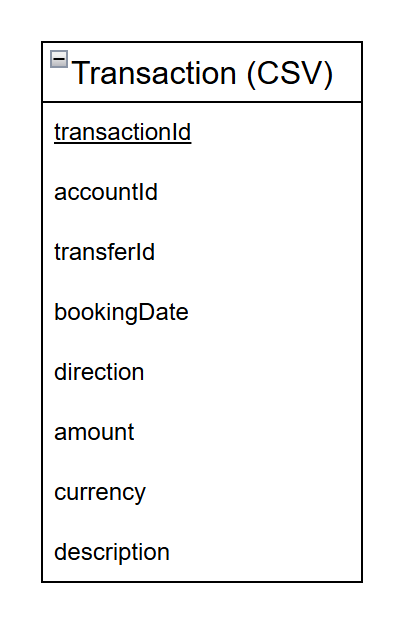
\includegraphics[width=0.32\textwidth,height=0.47\textheight,keepaspectratio]{images/logical-csv.png}
\caption{CSV logical model: transaction fields.}
\label{fig:logical-csv}
\end{figure}
\clearpage

\subsection{Physical models}

The MongoDB physical model specifies BSON types, required and optional
fields, validation rules and indexes. Reference arrows describe lookup paths;
MongoDB does not enforce foreign keys between collections. The executable
schema is maintained in \path{Diogo/database/schema.js}.

\begin{figure}[htbp]
\centering
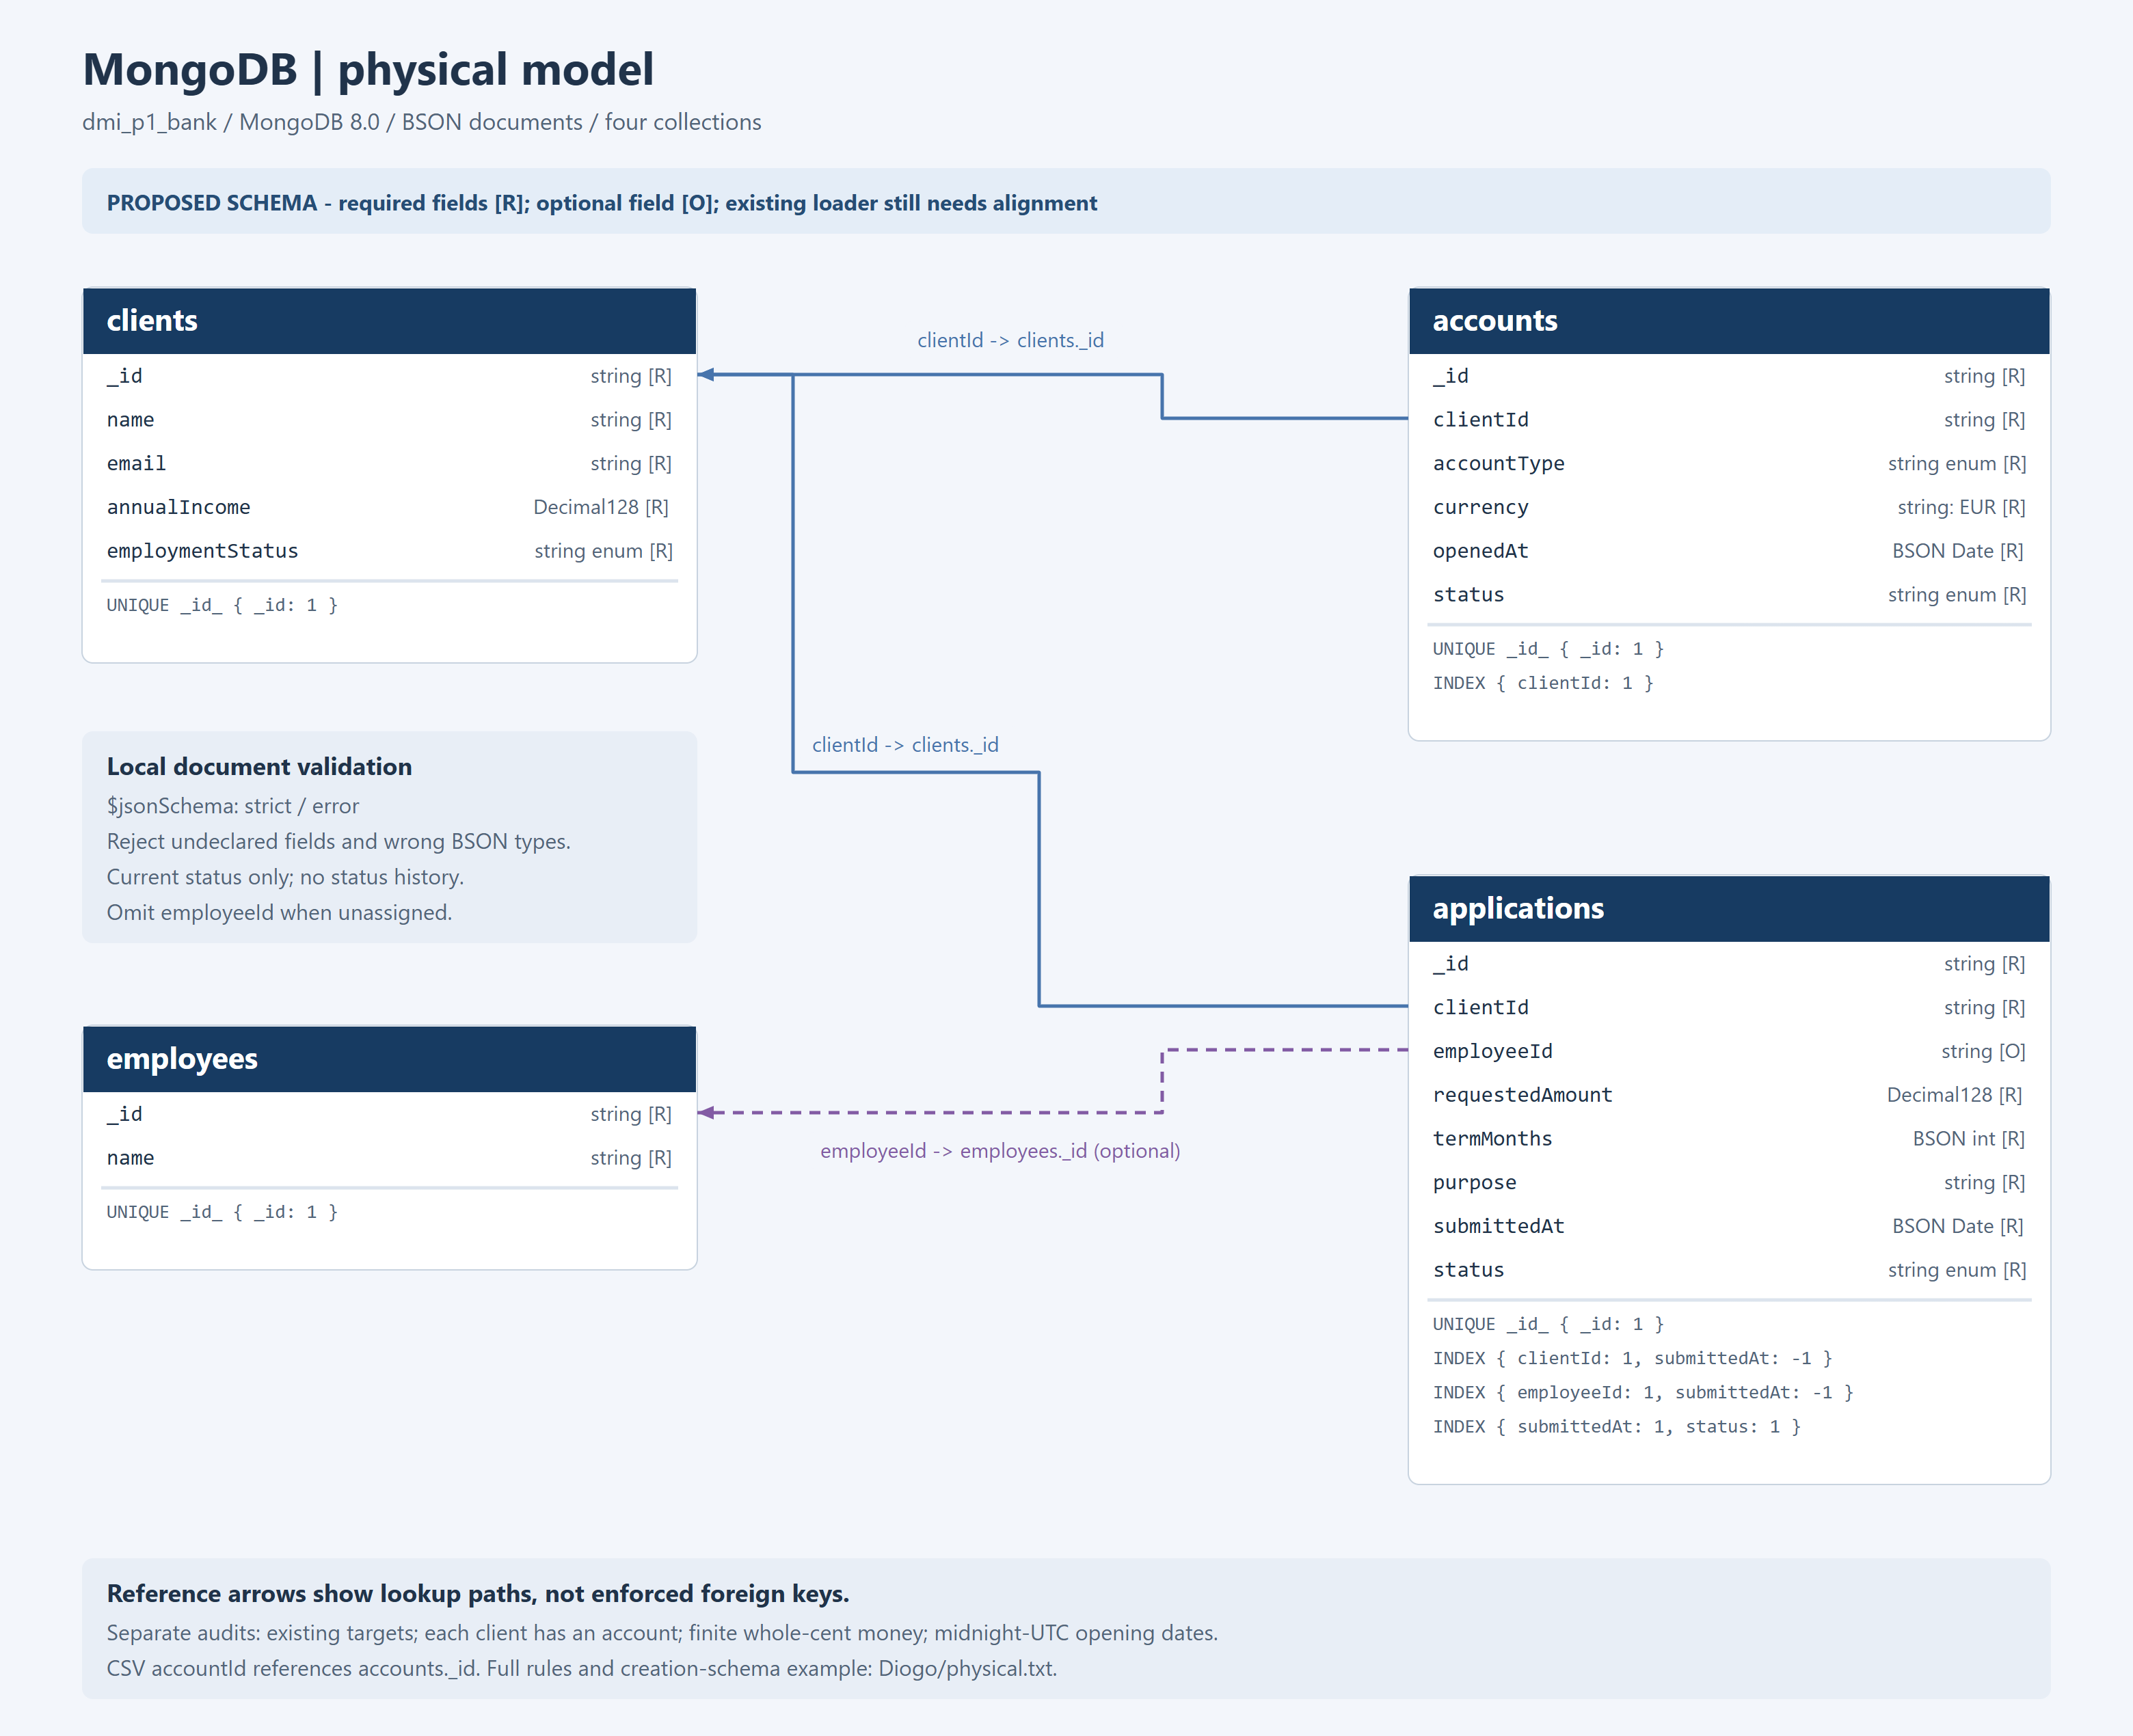
\includegraphics[width=\textwidth,height=0.78\textheight,keepaspectratio]{images/mongodb-physical.png}
\caption{MongoDB physical model: storage types, indexes and validation.}
\label{fig:physical-mongodb}
\end{figure}
\clearpage

The CSV physical model specifies column order, text representations,
encoding, delimiters and validation rules. Dates and amounts are stored as
text and parsed by the reader. Account references and transfer pairs require
validation outside the file format.

\begin{figure}[htbp]
\centering
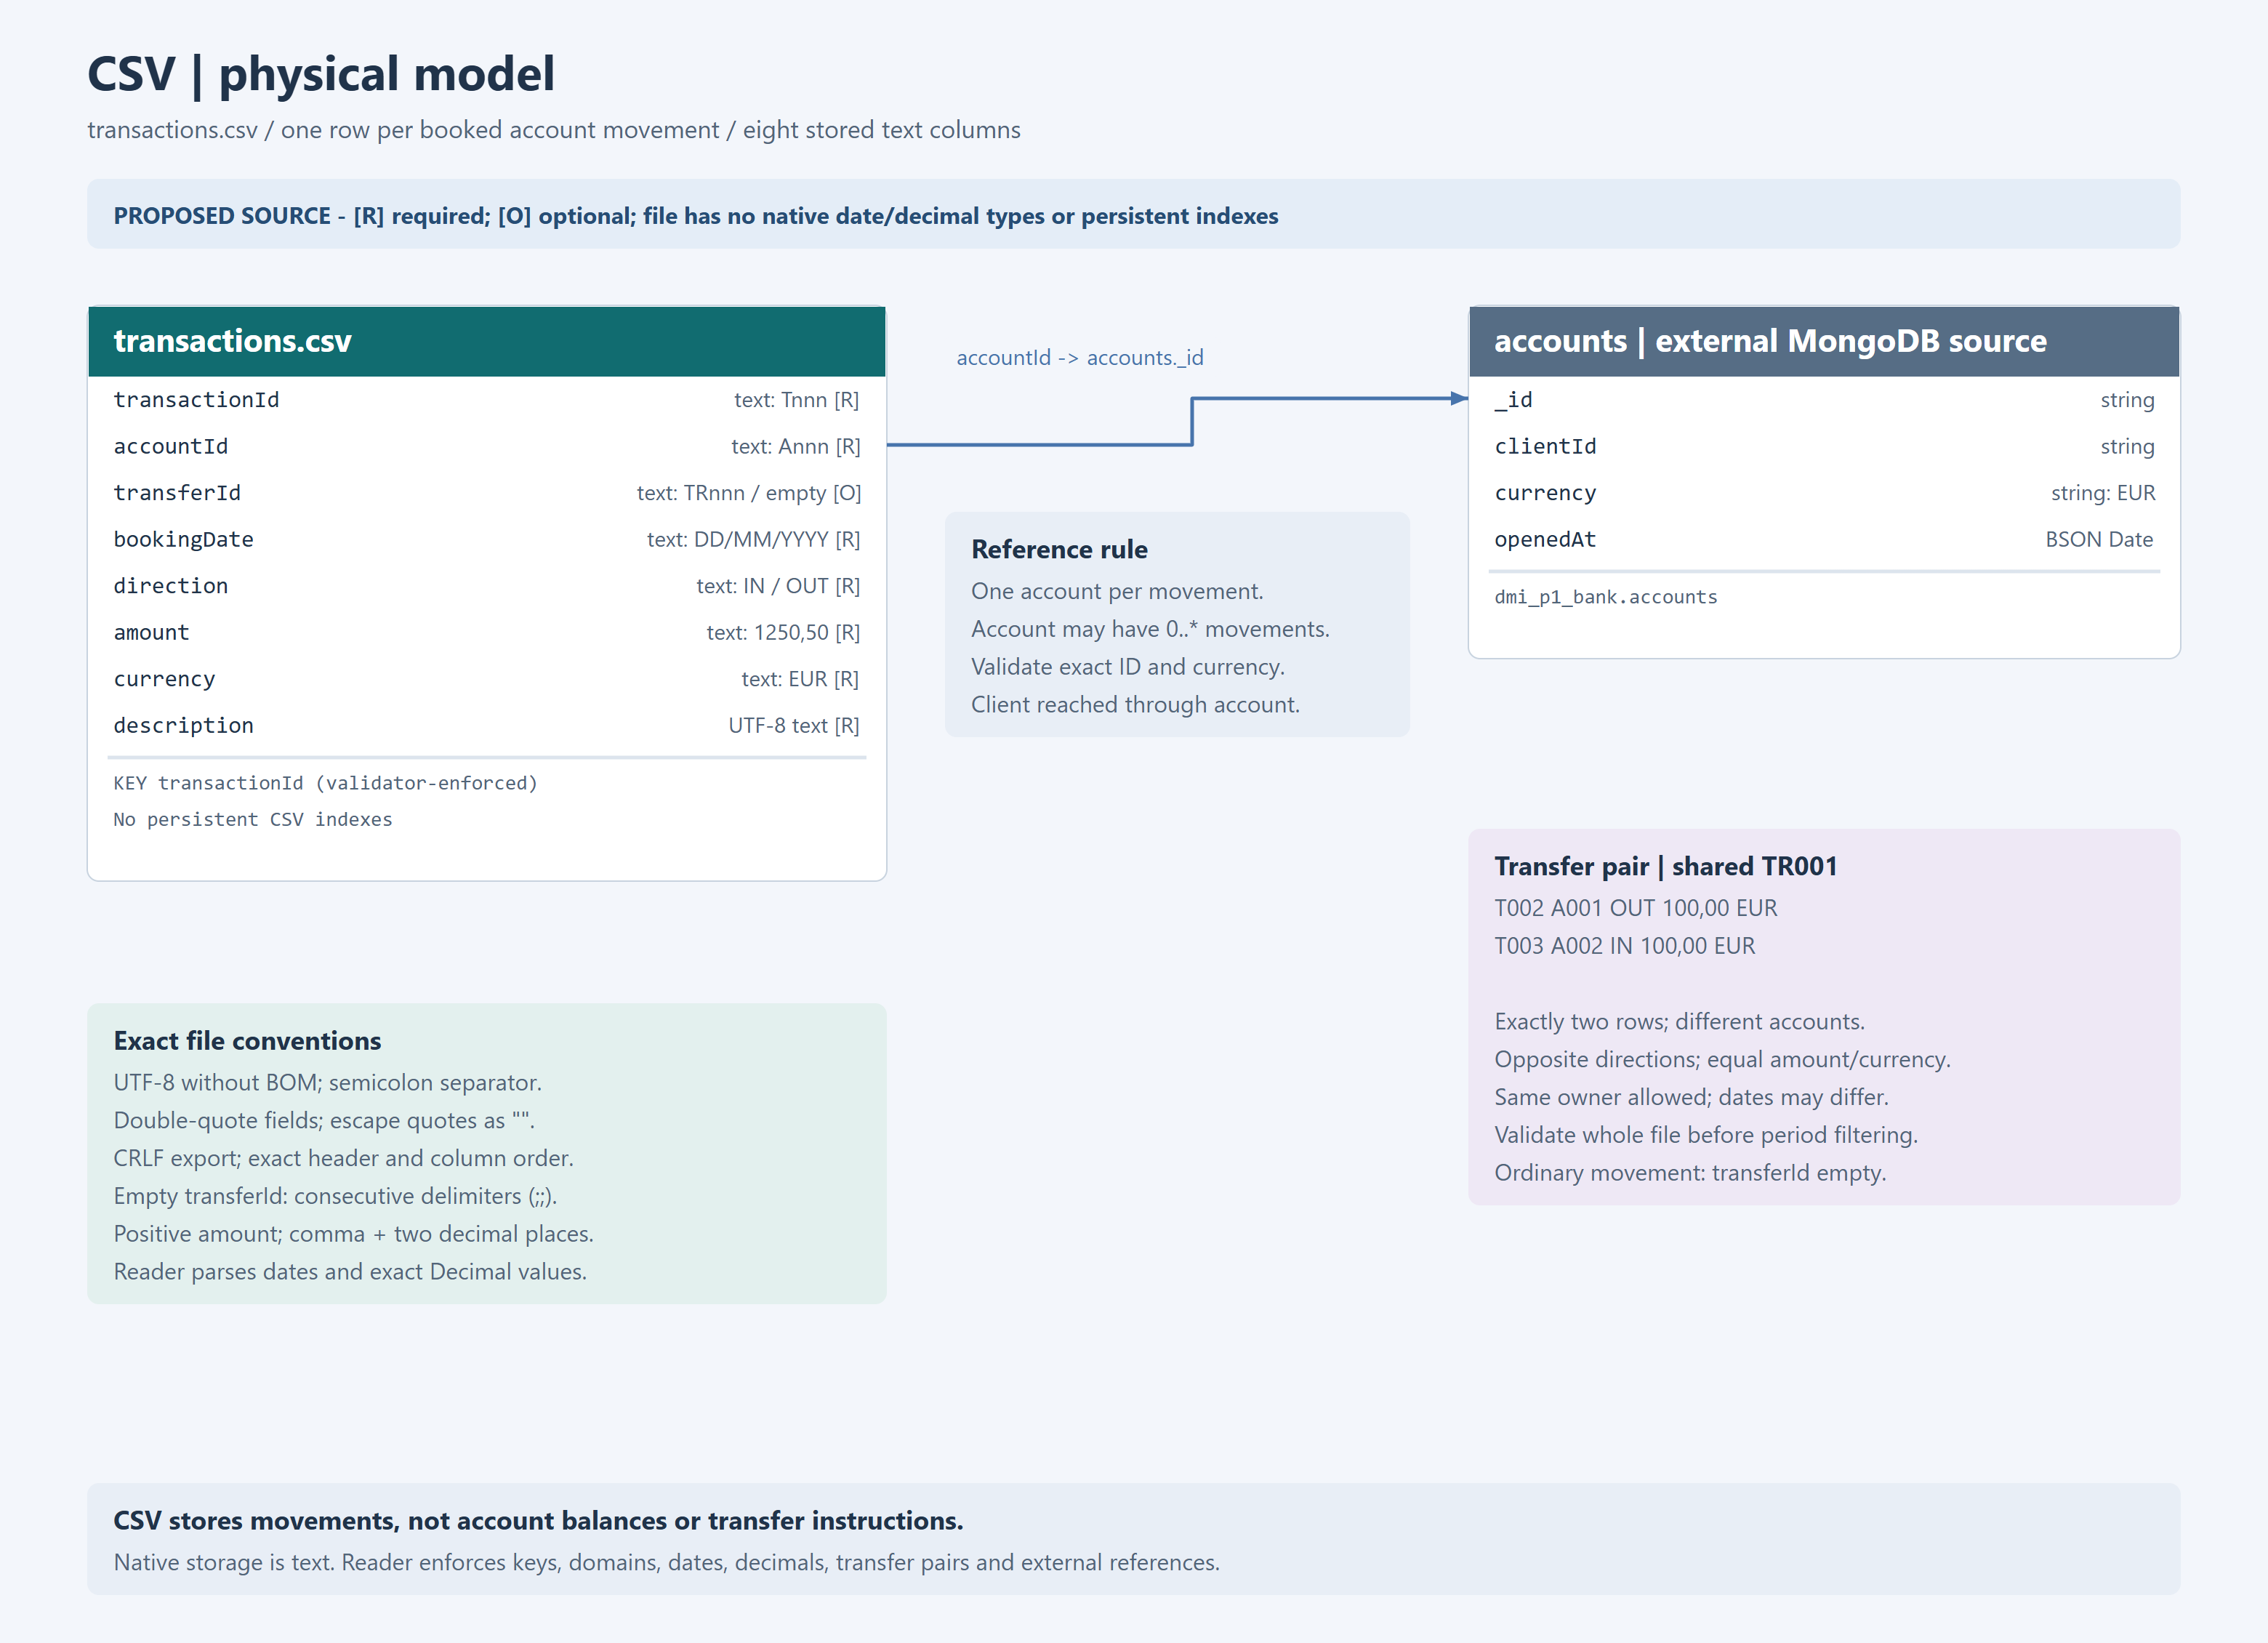
\includegraphics[width=\textwidth,height=0.78\textheight,keepaspectratio]{images/csv-physical.png}
\caption{CSV physical model: file conventions, account references and transfer pairs.}
\label{fig:physical-csv}
\end{figure}
\clearpage

\section{Data generation process and data quality analysis}

\subsection{Generation strategy}

The banking sources use synthetic generated data rather than real collected customer data.
The aim is to produce a coherent dataset large enough to demonstrate the
MongoDB and CSV models and their queries, while retaining deliberately
constructed cases with independently checkable results.

Values are generated locally by a Python script based on predefined values 
and a random number generator. AI assisted with the design and implementation 
of the process as well as value selection for the generator. All
records are then produced by running a simple python script. Generation requires Python's
standard library only; it does not call any external services or requires internet connection.
The generator is also deterministic so the same databases can be shared by simply sharing the 
original script

Two profiles are maintained separately. The reference profile contains five
clients, two employees, six accounts, six applications and ten transactions,
with hand-specified query answers. The scale profile provides the working
sources shown below. Reference and scale records and expected results must
not be mixed.

\begingroup
\renewcommand{\arraystretch}{1.2}
\begin{tabularx}{\textwidth}{@{}l r >{\raggedright\arraybackslash}X@{}}
\toprule
Source / entity & Records & Allocation rule\\
\midrule
MongoDB clients & 500 & Root population for ownership and applications.\\
MongoDB employees & 25 & Created before application assignment.\\
MongoDB accounts & 1,000 & 100 clients own one account, 300 own two and 100 own three.\\
MongoDB applications & 750 & Controlled distribution of occasional, repeat and non-applicants.\\
\textbf{MongoDB total} & \textbf{2,275} & Four collections.\\
CSV transactions & 8,000 & 6,000 ordinary movements and 1,000 two-record transfer pairs, plus one file header.\\
\bottomrule
\end{tabularx}
\endgroup

The process follows a dependency order: first clients are made, then employees,
then accounts, then credit applications and finally transactions. References are selected from the 
already existing records. There is a period selected of 1 January--31 October 2026, with 31 October 
as the snapshot date.

\subsection{Client, employee and account generation}

Scale identifiers use a type prefix and six zero-padded digits, for example
\texttt{C000001}, \texttt{E000001}, \texttt{A000001}, \texttt{L000001},
\texttt{T000001} and \texttt{TR000001}.

All names are created by sampling a catalogue of first names and surnames that were previously
generated. This list features 80 first names and 80 surnames with each full name
seleting one first name and two different surnames. 

Client emails are derived directly from the unique identifier for simplicity and to avoid
repeating names. For example, client \texttt{C000001} has the email \texttt{c000001@example.invalid}.
The invalid domain is selected to make obvious that the values are not real.

Employee emails are generated from the first name and surname, with a random number added as well to
avoid duplicates.

Employment categories use exact quotas. Within a category, the generator
selects an income area with a certain configured probability, then samples
uniformly in integer cents inside that same area.

Every client receices a current personal account. Additional accounts are 
generated randomly as well and may not exist, may be current also or may be savings accounts.
The probabilities of each type are 25\% for current and 75\% for savings. 

\begingroup
\renewcommand{\arraystretch}{1.2}
\begin{tabularx}{\textwidth}{@{}p{2.5cm} r >{\raggedright\arraybackslash}X p{2.4cm}@{}}
\toprule
Employment & Clients & Annual income bands (EUR) & Band weights\\
\midrule
Employed & 325 & 15,000--24,999.99; 25,000--44,999.99; 45,000--90,000 & 25\%, 55\%, 20\%\\
Self-employed & 50 & 8,000--19,999.99; 20,000--59,999.99; 60,000--140,000 & 25\%, 55\%, 20\%\\
Retired & 50 & 6,000--11,999.99; 12,000--24,999.99; 25,000--45,000 & 30\%, 55\%, 15\%\\
Student & 50 & Exactly zero; 0.01--6,000; 6,000.01--18,000 & 35\%, 45\%, 20\%\\
Unemployed & 25 & Exactly zero; 0.01--9,000; 9,000.01--18,000 & 45\%, 40\%, 15\%\\
\bottomrule
\end{tabularx}
\endgroup

\subsection{Credit application generation}

Applications distribution is sampled by exact values to support meaningful query cases:
150 clients have none, 200 have one, 75 have two, and 25 each have four, five, six
and seven applications.

Each application contains an identifier, existing client reference, requested
amount, repayment term, purpose, submission timestamp and current status.
The exact status quotas are 410 approved, 190 declined and 150 pending.
Exactly 75 pending applications are intentionally left without \texttt{employeeId};
every other request references an existing employee. One employee is reserved
with no assigned applications, while the remaining 24 receive assignments
with varying workloads.

\begingroup
\renewcommand{\arraystretch}{1.2}
\begin{tabularx}{\textwidth}{@{}p{3cm} r p{3cm} >{\raggedright\arraybackslash}X@{}}
\toprule
Purpose & Requests & Amount range (EUR) & Term choices (months)\\
\midrule
Vehicle & 260 & 3,000--45,000 & 12, 24, 36, 48, 60, 72\\
Education & 115 & 1,000--30,000 & 12, 24, 36, 48, 60, 84\\
Home improvement & 190 & 5,000--120,000 & 24, 36, 60, 84, 120, 180, 240\\
Personal expense & 110 & 500--20,000 & 6, 12, 24, 36, 48\\
Debt consolidation & 75 & 2,000--50,000 & 12, 24, 36, 48, 60, 84\\
\bottomrule
\end{tabularx}
\endgroup

Apart from the two fixed query examples, each request has a 60\% probability
of selecting a common amount from its purpose-specific list, such as
EUR 5,000, 10,000 or 25,000. Otherwise, an amount is sampled uniformly among
EUR 10 multiples within the purpose range, producing values such as
EUR 12,340.

Submission timestamps include a sampled time of day in UTC. Assigned pending
requests are dated August torugh October; unassigned pending requests are dated
16 trough 31 October. Approved and declined requests are dated January trough 15 October.
These date windows have been selected with the assistance of an AI model and
their purpose is to create a realistic snapshot of a bank credit application in
a moment in time.

Finally the status of each application is determined by a random number generator.

\subsection{Transaction generation}

All transaction fields are populated initially with the exception of
\texttt{transferId}, which is intentionally left empty. Each record has a unique
identifier, an existing account reference, booking date, direction, positive
amount, EUR currency and a description selected from frozen templates.
Dates cannot precede the referenced account's opening date. Purchases,
deposits and withdrawals use current accounts.

\begingroup
\renewcommand{\arraystretch}{1.2}
\begin{tabularx}{\textwidth}{@{}p{3cm} r >{\raggedright\arraybackslash}X@{}}
\toprule
Movement category & Rows & Generation rule\\
\midrule
Salary / pension & 1,800 & 150 employed and 30 retired clients receive monthly incoming movements each.\\
Deposits & 200 & Incoming amounts from EUR 20 to 10,000.\\
Purchases & 3,000 & Outgoing amounts from EUR 0.50 to 5,000.\\
Withdrawals & 500 & Outgoing amounts from EUR 10 to 500, in EUR 10 increments.\\
Fees & 500 & Outgoing amounts from EUR 0.50 to 15.\\
Transfer movements & 2,000 & 1,000 pairs, with amounts from EUR 1 to 20,000 per pair.\\
\bottomrule
\end{tabularx}
\endgroup

Recurring income is booked on day 25 of each month. Its base is annual income
divided by 12, rounded half-up to cents.

Each transfer is generated as one unit containing two records on different
accounts: one \texttt{OUT} and one \texttt{IN}, sharing a transfer identifier,
amount, currency and booking date. There are exactly 300 same-client pairs
and 700 pairs between different clients. Both accounts must already exist
and be open by the booking date.

Other special scenarios include clients with no movements, accounts with no
movements, clients with no September activity, and records dated 31 August,
1 September, 30 September and 1 October. These dates test inclusion and
exclusion at the query-period boundaries. Accented characters, embedded
quotes, semicolons, cent amounts and repeated descriptions exercise parsing
and aggregation without introducing invalid records into the main sources.

\subsection{Reproducibility, interruption recovery and exports}

The completed runs used generator version 1.1.0, base seed 42, CPython 3.14.3
and SQLite 3.50.4. Stable stage and unit seeds make record values independent
of batch size and interruption position.

\subsection{Data quality checks and measured results}

The values have been manually verified against the initial rules and evaluated
on whether or not they are coherent and possibly meaningful.

A separate validation module re-reads the actual exported files rather than
accepting successful record construction as evidence of quality. It checks
a list of rules previously defined for the generation process and reports any mistake
or finished with no error sucessfully.

\section{Queries and expected results}
This section defined two queries for the banking subtopic, query Q1 is defined as
a simple query and query Q2 is defined as an intermiate query.

\subsection{Q1: Customer credit applications -- simple}
Which applications did C004 submit, and what are their amounts and statuses?

This uses filtering, projection and ordering within one collection inside the MongoDB source only

\begin{lstlisting}
bank.applications.find(
  { clientId: 'C004' },
  { _id: 1, requestedAmount: 1, status: 1 }
).sort({ _id: 1 })
\end{lstlisting}
\begin{center}
\begin{tabular}{l r l}
\toprule
Application & Requested amount (EUR) & Status\\\midrule
L004 & 18000 & pending\\
L005 & 32000 & declined\\\bottomrule
\end{tabular}
\end{center}
C005 must return an empty result, not an error.

\subsection{Q2: Customer movement totals -- intermediate}

For each client, what are the total incoming and outgoing account movements
from 1 to 30 September 2026, across all their accounts, including clients
with no movements?

This query combines MongoDB's \texttt{clients} and \texttt{accounts}
collections with the CSV transaction source. Account ownership is resolved
through \texttt{accounts.clientId = clients.\_id}; transactions are linked
through \texttt{transactions.accountId = accounts.\_id}.

The following extended expression specifies the complete query.

To run it we need a CSV wrapper that reads the CSV file and exposes all
the recores included.

\begin{lstlisting}
SeptemberMovement(C, T, Dir, M) :-
    Client(C),
    Account(K, C),
    Transaction(T, K, D, Dir, M, "EUR"),
    D >= "2026-09-01",
    D <= "2026-09-30".

Incoming(C, T, M) :- SeptemberMovement(C, T, "IN", M).
Outgoing(C, T, M) :- SeptemberMovement(C, T, "OUT", M).

HasIncoming(C) :- Incoming(C, T, M).
HasOutgoing(C) :- Outgoing(C, T, M).

IncomingTotal(C, sum<M>) :- Incoming(C, T, M).
OutgoingTotal(C, sum<M>) :- Outgoing(C, T, M).

IncomingTotal(C, 0.00) :- Client(C), not HasIncoming(C).
OutgoingTotal(C, 0.00) :- Client(C), not HasOutgoing(C).

Q2(C, TotalIn, TotalOut) :-
    Client(C),
    IncomingTotal(C, TotalIn),
    OutgoingTotal(C, TotalOut).
\end{lstlisting}


\begingroup
\renewcommand{\arraystretch}{1.2}
\begin{tabularx}{\textwidth}{@{}l r r@{}}
\toprule
Client & Total incoming (EUR) & Total outgoing (EUR)\\
\midrule
C000001 & 18804.03 & 3794.96\\
C000002 & 0.00 & 736.22\\
C000003 & 0.00 & 19592.04\\
C000004 & 0.00 & 2780.85\\
C000005 & 0.00 & 0.00\\
\bottomrule
\end{tabularx}
\endgroup

The table shows the first five expected rows of the scale dataset. 
The complete expected result contains 500 rows,
one per client, and is stored in that run's
\texttt{expected-query-results.json}. Across all clients, September's expected
incoming total is EUR 2,130,127.13 and outgoing total is EUR 2,383,262.07.
These values were calculated from the exported sources by the independent
validation module; they are not evidence of executing the cross-source query.

Both date boundaries are inclusive. 

Transfers contribute to the totals of their respective accounts, 
a same-client transfer contributes once to that
client's incoming total and once to the outgoing total. 

\section{Initial heterogeneity and integration plan}
The proposed CSV contract uses UTF-8, semicolon separators and columns
\texttt{movement\_id}, \texttt{account\_id}, \texttt{booking\_date},
\texttt{direction}, \texttt{amount}, \texttt{currency}. Dates use
\texttt{DD/MM/YYYY}, direction uses \texttt{IN}/\texttt{OUT}, amounts use a
decimal comma without thousands separators, and all amounts are positive EUR.

Below we we have a list of possile conflicts betweens sources and the proposed future integration rules to
allow for a coherent complete model.

\begin{tabularx}{\textwidth}{@{}l X X@{}}
\toprule
Conflict & Source representations & Proposed P2 rule\\\midrule
Structural & Nested MongoDB documents versus flat CSV rows & Expose Client,
Account, Application and Movement entities in a global model.\\
Syntactic & BSON date versus CSV day/month/year & Parse CSV strictly as a
calendar date; retain distinction from UTC event timestamps.\\
Syntactic & Decimal128 versus comma-decimal text & Parse exact decimal values;
avoid binary floating-point arithmetic.\\
Semantic & CSV IN/OUT movement direction & Map to incoming/outgoing; preserve
positive amount and explicit currency.\\
Naming & \texttt{\_id} versus \texttt{account\_id} & Map to global accountId
after validating references.\\
\bottomrule
\end{tabularx}
Cross-subtopic identity resolution needs an agreed organisation or
identifier structure. Matching solely by names is not acceptable for these domains.
No mapping to any investment/fintech sources will be defined until the complete
schema of both contracts are known and understood.

\section{Installation and execution}

All files required for Diogo's banking sources are contained in the
\texttt{Diogo} folder. Docker Compose configuration is supplied in
\texttt{compose.yaml}; it starts MongoDB and the mongo-express browser viewer.
Prerequisites are Docker Desktop with its Linux engine running and Python
3.11 or later. No additional Python packages.

From the \texttt{Diogo} folder, run:
\begin{lstlisting}
docker compose up -d --wait
python -B dataGeneration/generate.py run --profile scale
python -B database/load.py
python -B queries/execute.py
\end{lstlisting}

The commands start the services, generate the dataset,
load and verify MongoDB, and execute both queries. MongoDB has a readiness
check, and the data is persisted in a Docker volume.The transactions CSV
is contained in a a separate file.

Documents can be viewed at \url{http://127.0.0.1:8081}, or in MongoDB Compass (if installed)
using \texttt{mongodb://127.0.0.1:27017/}. The database is
\texttt{dmi\_p1\_bank}. To stop services while retaining stored data, use
\texttt{docker compose stop}.

The query runner reads the live MongoDB source and validates the matching
CSV and source manifest. Q1 executes in MongoDB only, while Q2 joins live
account ownership to CSV transactions in Python.
The runner compares every result row against the saved expected answers and
prints \texttt{PASS} only when both queries match. Results are saved in
\path{queries/results/scale-results.json}; the complete Q2 table is also
saved in \path{queries/results/scale-q2.csv}. Paths in this section are
relative to \texttt{Diogo}.

\subsection{Q1: Actual execution result}

The live query returned:

\begingroup
\renewcommand{\arraystretch}{1.2}
\begin{tabularx}{\textwidth}{@{}l r >{\raggedright\arraybackslash}X@{}}
\toprule
Application & Requested amount (EUR) & Status\\
\midrule
L000004 & 18000.00 & pending\\
L000005 & 32000.00 & declined\\
\bottomrule
\end{tabularx}
\endgroup

Both rows matched the expected result. These are the scale-profile
identifiers corresponding to the shorter reference identifiers used in the
initial examples.

\subsection{Q2: Actual execution result}

Q2 processed 930 matching movements and returned exactly 500 rows, one per
client, as predicted. The first five actual rows are:

\begingroup
\renewcommand{\arraystretch}{1.2}
\begin{tabularx}{\textwidth}{@{}l r r@{}}
\toprule
Client & Total incoming (EUR) & Total outgoing (EUR)\\
\midrule
C000001 & 18804.03 & 3794.96\\
C000002 & 0.00 & 736.22\\
C000003 & 0.00 & 19592.04\\
C000004 & 0.00 & 2780.85\\
C000005 & 0.00 & 0.00\\
\bottomrule
\end{tabularx}
\endgroup

The output retains 121 clients with zero September activity. 
Across all clients, actual incoming
movements total EUR 2,130,127.13 and outgoing movements total
EUR 2,383,262.07.

\section{Cross-subtopic queries for P2}

The following eight natural-language queries define the proposed integration
work for P2. Together with the four existing individual queries, they form
the twelve-query set required in P1. Diogo's existing queries are simple and
intermediate; Oleksii's are classified as intermediate and complex.
The additional queries therefore comprise three simple, two intermediate
and three complex queries, giving four of each difficulty overall.

\begingroup
\renewcommand{\arraystretch}{1.2}
\begin{longtable}{@{}p{0.8cm} p{2.2cm} p{\dimexpr\textwidth-3cm-4\tabcolsep\relax}@{}}
\toprule
ID & Difficulty & Natural-language query\\
\midrule
\endfirsthead
\toprule
ID & Difficulty & Natural-language query (continued)\\
\midrule
\endhead
\bottomrule
\endfoot

G1 & Simple &
For a selected startup, list its linked banking clients and their active
accounts, showing the startup name, client name, account identifier and
account type.\\

G2 & Simple &
For a selected startup, list the pending credit applications submitted by
its linked banking clients, showing each client, application identifier,
requested amount and submission date.\\

G3 & Simple &
For a selected reporting month and MRR threshold, list startups whose
reported MRR exceeds that threshold and that have a linked banking client
with an active current account. Show the startup, reported MRR and
matching client and account identifiers.\\

G4 & Intermediate &
For each startup, calculate the total incoming and outgoing movements
across the accounts of its linked banking clients during a selected period.
Include startups with no matching movements with zero totals.\\

G5 & Intermediate &
For each startup sector and application status, calculate the number and
total requested amount of credit applications submitted during a selected
period by linked banking clients. Count each application only once within
each sector, even if its client is associated with several startups in that
sector.\\

G6 & Complex &
Between two selected consecutive reporting months, identify startups whose
MRR increased while their linked clients' combined net account movement
(incoming minus outgoing) decreased. Show both monthly MRR values, the MRR
growth percentage and both net movement totals.\\

G7 & Complex &
For funding rounds in a selected period, identify those with no incoming
movement on any linked client's account matching the funding amount in a
common currency within 30 days before or after the round date. Show the
startup, investor, round date and amount for manual review of the potential
correspondence.\\

G8 & Complex &
Rank investor funds by the number of distinct portfolio startups whose MRR
decreased between two selected consecutive reporting months and whose
linked banking clients had at least one declined credit application during
the later month. Show the qualifying startup count and total funding recorded
for those startups from each fund, without duplicating rounds or startups
because of multiple clients, accounts or applications.\\

\end{longtable}
\endgroup

\end{document}
